\documentclass[12pt,a4paper]{article}

\usepackage[a4paper,margin=1in]{geometry}
\usepackage[T1]{fontenc}
\usepackage[utf8]{inputenc}
\usepackage{xcolor}
\usepackage{tikz}
\usepackage{booktabs}
\usepackage{array}
\usepackage{float}
\usepackage{tabularx}
\usepackage{enumitem}
\usetikzlibrary{arrows.meta, positioning, shapes.geometric, shapes.multipart, shadows, fit, backgrounds, calc}

\DeclareRobustCommand{\code}[1]{\texttt{\detokenize{#1}}}
\setlength{\emergencystretch}{4em}

% Copy these colors/styles into main.tex if they are not already present.
\definecolor{layerDialogue}{RGB}{232,242,255}
\definecolor{layerGrounding}{RGB}{255,245,230}
\definecolor{layerPlanner}{RGB}{235,249,240}
\definecolor{layerExec}{RGB}{245,232,255}
\definecolor{layerSkill}{RGB}{242,242,242}
\definecolor{layerFuture}{RGB}{255,240,240}
\definecolor{lineMain}{RGB}{43,63,92}
\definecolor{lineFeedback}{RGB}{130,88,35}
\definecolor{lineEvidence}{RGB}{184,100,24}

\tikzset{
  thesisNode/.style={
    rounded corners=2pt,
    draw=lineMain!75,
    very thick,
    align=center,
    inner xsep=5pt,
    inner ysep=5pt,
    minimum height=8mm,
    font=\scriptsize,
    fill=white,
    drop shadow={shadow xshift=0.5pt, shadow yshift=-0.5pt, opacity=0.14}
  },
  dialogueNode/.style={thesisNode, fill=layerDialogue},
  groundingNode/.style={thesisNode, fill=layerGrounding},
  plannerNode/.style={thesisNode, fill=layerPlanner},
  execNode/.style={thesisNode, fill=layerExec},
  skillNode/.style={thesisNode, fill=layerSkill},
  futureNode/.style={thesisNode, dashed, fill=layerFuture},
  thesisFlow/.style={-{Latex[length=2.5mm,width=1.6mm]}, very thick, draw=lineMain},
  evidenceFlow/.style={-{Latex[length=2.2mm,width=1.4mm]}, thick, draw=lineEvidence},
  feedbackFlow/.style={-{Latex[length=2.2mm,width=1.4mm]}, thick, draw=lineFeedback, dashed},
  layerBox/.style={rounded corners=3pt, draw=lineMain!35, thick, inner sep=7pt}
}

\begin{document}

% ---------------------------------------------------------------------------
% Block 1: high-level implementation / stack visualization.
% Paste this near the start of Section 5, after the package role table.
% ---------------------------------------------------------------------------

\begin{figure}[H]
\centering
\resizebox{\linewidth}{!}{%
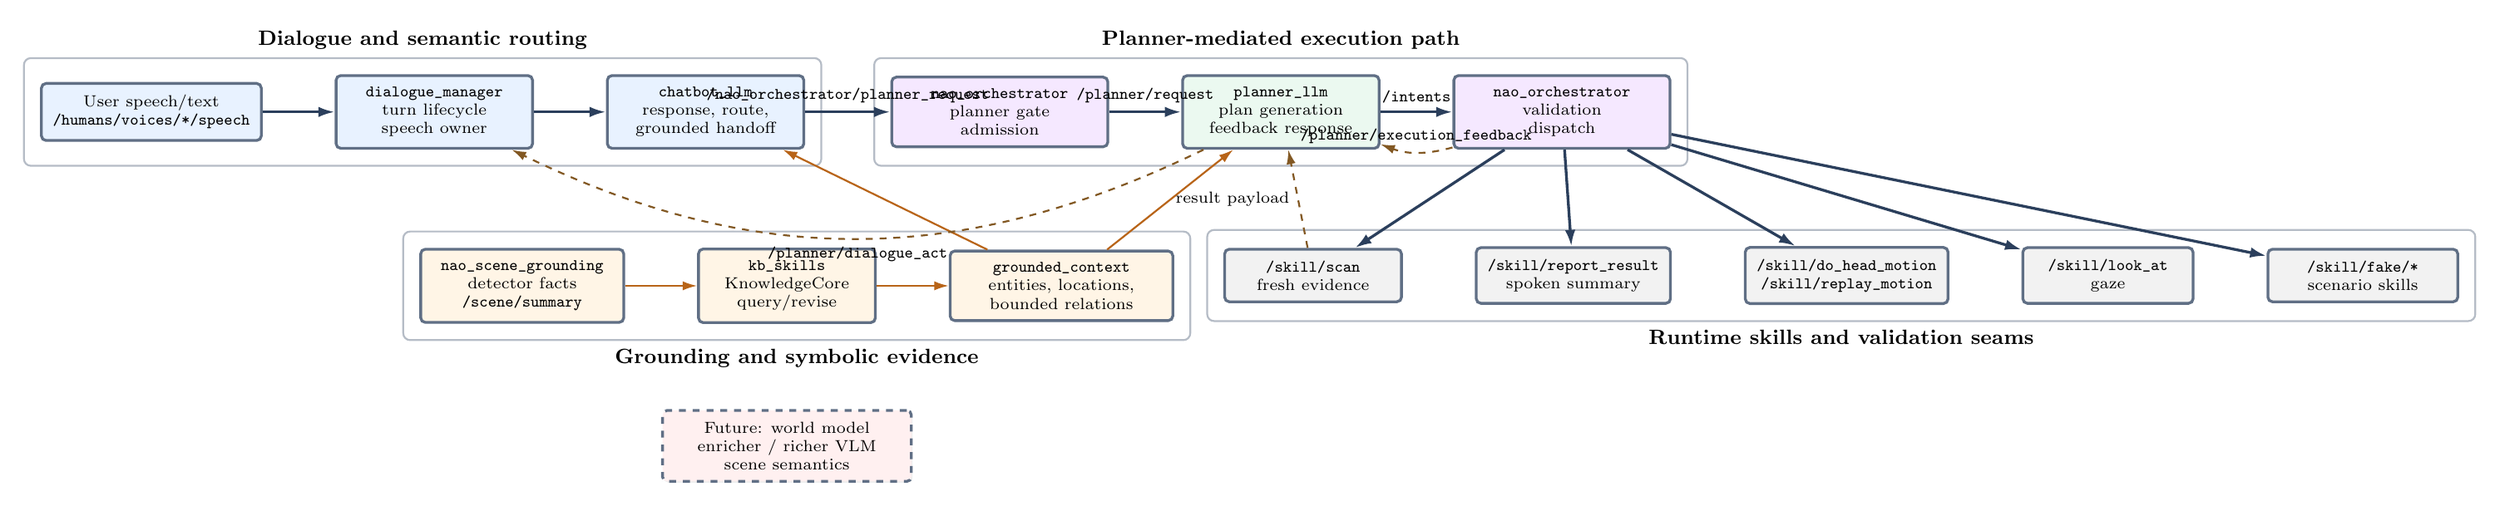
\begin{tikzpicture}[node distance=8mm and 11mm]
  \node[dialogueNode, minimum width=30mm] (user) {User speech/text\\\code{/humans/voices/*/speech}};
  \node[dialogueNode, right=of user, minimum width=30mm] (dm) {\code{dialogue_manager}\\turn lifecycle\\speech owner};
  \node[dialogueNode, right=of dm, minimum width=30mm] (chatbot) {\code{chatbot_llm}\\response, route,\\grounded handoff};

  \node[execNode, right=13mm of chatbot, minimum width=33mm] (gate) {\code{nao_orchestrator}\\planner gate\\admission};
  \node[plannerNode, right=of gate, minimum width=30mm] (planner) {\code{planner_llm}\\plan generation\\feedback response};
  \node[execNode, right=of planner, minimum width=33mm] (orch) {\code{nao_orchestrator}\\validation\\dispatch};

  \node[skillNode, below=15mm of orch, xshift=-38mm, minimum width=27mm] (scan) {\code{/skill/scan}\\fresh evidence};
  \node[skillNode, right=of scan, minimum width=29mm] (report) {\code{/skill/report_result}\\spoken summary};
  \node[skillNode, right=of report, minimum width=28mm] (motion) {\code{/skill/do_head_motion}\\\code{/skill/replay_motion}};
  \node[skillNode, right=of motion, minimum width=26mm] (look) {\code{/skill/look_at}\\gaze};
  \node[skillNode, right=of look, minimum width=29mm] (fake) {\code{/skill/fake/*}\\scenario skills};

  \node[groundingNode, below=15mm of chatbot, xshift=-28mm, minimum width=31mm] (ground) {\code{nao_scene_grounding}\\detector facts\\\code{/scene/summary}};
  \node[groundingNode, right=of ground, minimum width=27mm] (kb) {\code{kb_skills}\\KnowledgeCore\\query/revise};
  \node[groundingNode, right=of kb, minimum width=34mm] (context) {\code{grounded_context}\\entities, locations,\\bounded relations};

  \node[futureNode, below=13mm of kb, minimum width=38mm] (wme) {Future: world model\\enricher / richer VLM\\scene semantics};

  \draw[thesisFlow] (user) -- (dm);
  \draw[thesisFlow] (dm) -- (chatbot);
  \draw[thesisFlow] (chatbot) -- node[above, font=\scriptsize]{\code{/nao_orchestrator/planner_request}} (gate);
  \draw[thesisFlow] (gate) -- node[above, font=\scriptsize]{\code{/planner/request}} (planner);
  \draw[thesisFlow] (planner) -- node[above, font=\scriptsize]{\code{/intents}} (orch);

  \draw[thesisFlow] (orch) -- (scan);
  \draw[thesisFlow] (orch) -- (report);
  \draw[thesisFlow] (orch) -- (motion);
  \draw[thesisFlow] (orch) -- (look);
  \draw[thesisFlow] (orch) -- (fake);

  \draw[evidenceFlow] (ground) -- (kb);
  \draw[evidenceFlow] (kb) -- (context);
  \draw[evidenceFlow] (context) -- (chatbot);
  \draw[evidenceFlow] (context) -- (planner);

  \draw[feedbackFlow] (scan) -- node[left, font=\scriptsize]{result payload} (planner);
  \draw[feedbackFlow] (orch) to[bend left=18] node[above, font=\scriptsize]{\code{/planner/execution_feedback}} (planner);
  \draw[feedbackFlow] (planner) to[bend left=26] node[below, font=\scriptsize]{\code{/planner/dialogue_act}} (dm);

  \begin{pgfonlayer}{background}
    \node[layerBox, fit=(user)(dm)(chatbot), label={[font=\small\bfseries]above:Dialogue and semantic routing}] {};
    \node[layerBox, fit=(gate)(planner)(orch), label={[font=\small\bfseries]above:Planner-mediated execution path}] {};
    \node[layerBox, fit=(ground)(kb)(context), label={[font=\small\bfseries]below:Grounding and symbolic evidence}] {};
    \node[layerBox, fit=(scan)(report)(motion)(look)(fake), label={[font=\small\bfseries]below:Runtime skills and validation seams}] {};
  \end{pgfonlayer}
\end{tikzpicture}%
}
\caption{Implemented ROS4HRI planner stack. Dialogue, planning, deterministic execution, symbolic grounding, and runtime skills remain separate owners. Dashed boxes mark future implementation directions rather than current execution authority.}
\label{fig:implementation-stack}
\end{figure}

% ---------------------------------------------------------------------------
% Block 2: compact runtime loop diagram.
% ---------------------------------------------------------------------------

\begin{figure}[H]
\centering
\resizebox{\linewidth}{!}{%
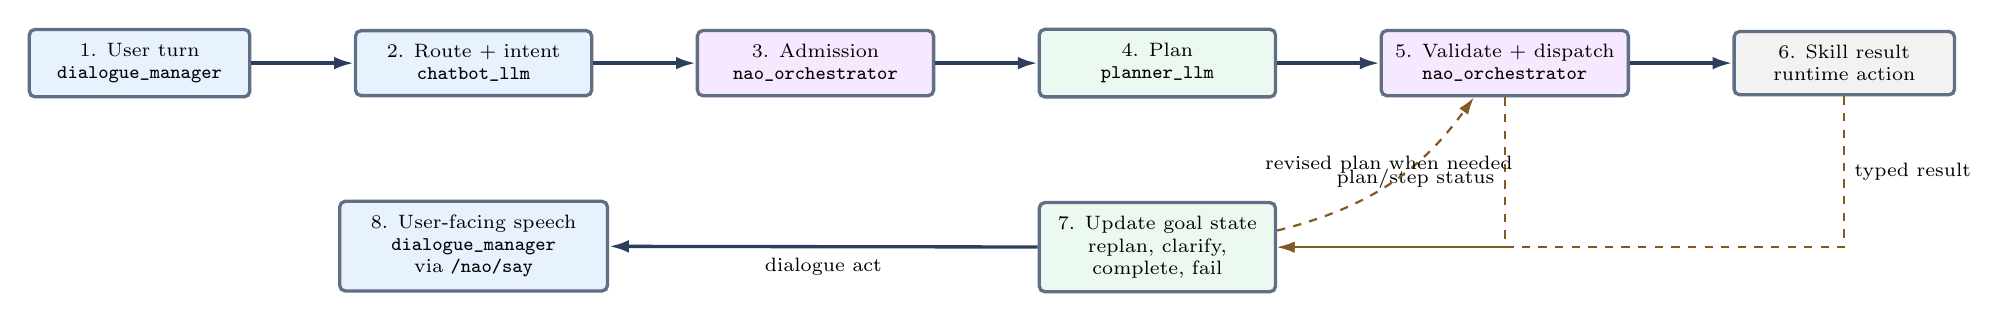
\begin{tikzpicture}[node distance=9mm and 13mm]
  \node[dialogueNode, minimum width=28mm] (turn) {1. User turn\\\code{dialogue_manager}};
  \node[dialogueNode, right=of turn, minimum width=30mm] (route) {2. Route + intent\\\code{chatbot_llm}};
  \node[execNode, right=of route, minimum width=30mm] (admit) {3. Admission\\\code{nao_orchestrator}};
  \node[plannerNode, right=of admit, minimum width=30mm] (plan) {4. Plan\\\code{planner_llm}};
  \node[execNode, right=of plan, minimum width=31mm] (validate) {5. Validate + dispatch\\\code{nao_orchestrator}};
  \node[skillNode, right=of validate, minimum width=28mm] (skill) {6. Skill result\\runtime action};

  \node[plannerNode, below=13mm of plan, minimum width=30mm] (statehelper) {7. Update goal state\\replan, clarify,\\complete, fail};
  \node[dialogueNode, below=13mm of route, minimum width=34mm] (speak) {8. User-facing speech\\\code{dialogue_manager}\\via \code{/nao/say}};

  \draw[thesisFlow] (turn) -- (route);
  \draw[thesisFlow] (route) -- (admit);
  \draw[thesisFlow] (admit) -- (plan);
  \draw[thesisFlow] (plan) -- (validate);
  \draw[thesisFlow] (validate) -- (skill);
  \draw[feedbackFlow] (skill) |- node[pos=0.25, right, font=\scriptsize]{typed result} (statehelper);
  \draw[feedbackFlow] (validate) |- node[pos=0.27, left, font=\scriptsize]{plan/step status} (statehelper);
  \draw[thesisFlow] (statehelper) -- node[below, font=\scriptsize]{dialogue act} (speak);
  \draw[feedbackFlow] (statehelper) to[bend right=20] node[above, font=\scriptsize]{revised plan when needed} (validate);
\end{tikzpicture}%
}
\caption{Planner loop used by the implemented stack. The executor reports status and evidence; it does not invent replacement plans or final wording.}
\label{fig:planner-loop-implementation}
\end{figure}

% ---------------------------------------------------------------------------
% Block 3: validation evidence ladder for Sections 6--8.
% ---------------------------------------------------------------------------

\begin{figure}[H]
\centering
\resizebox{0.92\linewidth}{!}{%
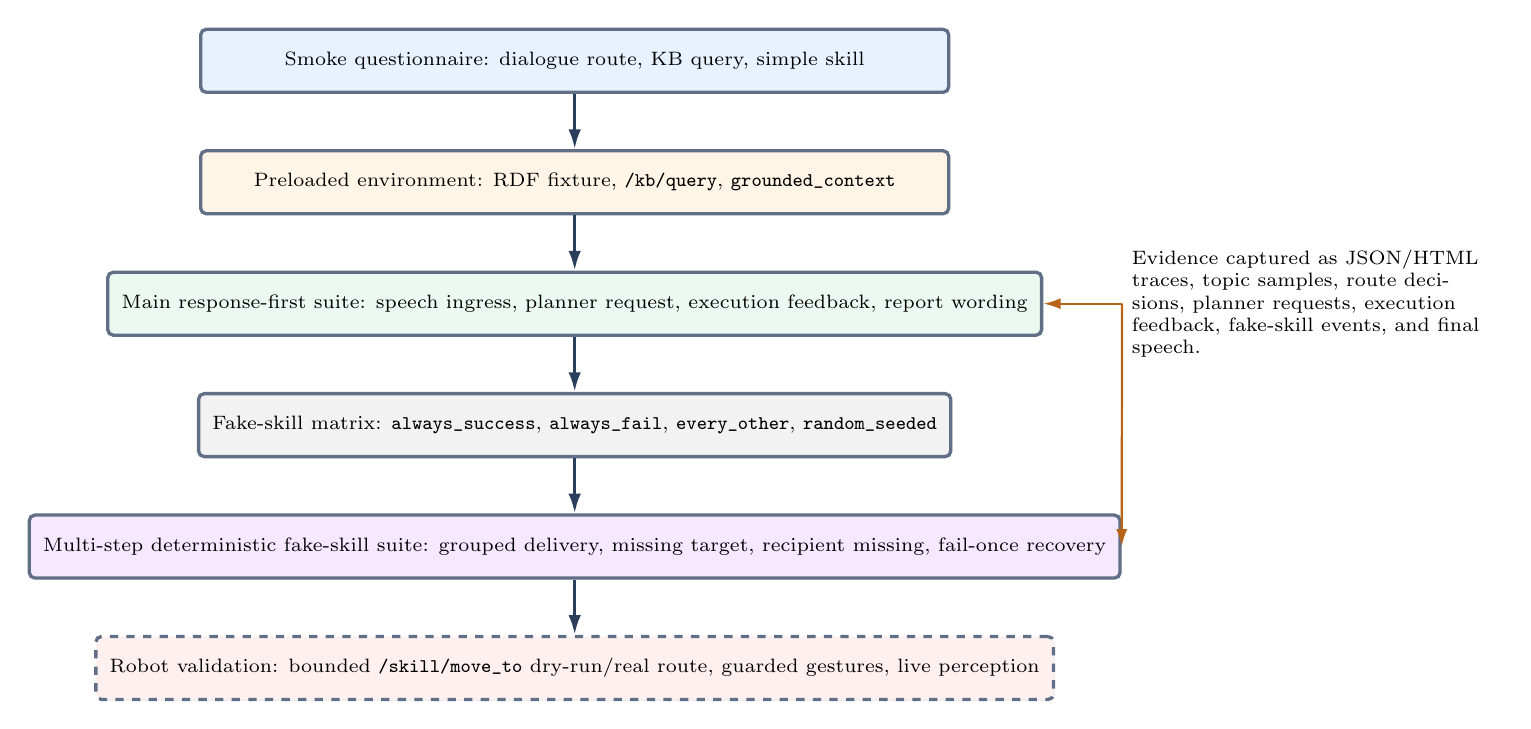
\begin{tikzpicture}[node distance=7mm]
  \node[dialogueNode, minimum width=95mm] (smoke) {Smoke questionnaire: dialogue route, KB query, simple skill};
  \node[groundingNode, below=of smoke, minimum width=95mm] (env) {Preloaded environment: RDF fixture, \code{/kb/query}, \code{grounded_context}};
  \node[plannerNode, below=of env, minimum width=95mm] (main) {Main response-first suite: speech ingress, planner request, execution feedback, report wording};
  \node[skillNode, below=of main, minimum width=95mm] (fake) {Fake-skill matrix: \code{always_success}, \code{always_fail}, \code{every_other}, \code{random_seeded}};
  \node[execNode, below=of fake, minimum width=95mm] (deep) {Multi-step deterministic fake-skill suite: grouped delivery, missing target, recipient missing, fail-once recovery};
  \node[futureNode, below=of deep, minimum width=95mm] (robot) {Robot validation: bounded \code{/skill/move_to} dry-run/real route, guarded gestures, live perception};

  \draw[thesisFlow] (smoke) -- (env);
  \draw[thesisFlow] (env) -- (main);
  \draw[thesisFlow] (main) -- (fake);
  \draw[thesisFlow] (fake) -- (deep);
  \draw[thesisFlow] (deep) -- (robot);

  \node[align=left, font=\scriptsize, right=10mm of main, text width=46mm] (notes)
  {Evidence captured as JSON/HTML traces, topic samples, route decisions, planner requests, execution feedback, fake-skill events, and final speech.};
  \draw[evidenceFlow] (notes.west) -- (main.east);
  \draw[evidenceFlow] (notes.west) -- (deep.east);
\end{tikzpicture}%
}
\caption{Validation ladder used to separate stable thesis evidence from harder replan and real-robot promotion claims.}
\label{fig:validation-ladder}
\end{figure}

% ---------------------------------------------------------------------------
% Block 4: implementation prose to replace the current Section 5 TODO bullets.
% ---------------------------------------------------------------------------

\section*{Implementation Prose Blocks}

\subsection*{\code{dialogue_manager}}

\code{dialogue_manager} is the dialogue turn owner and the final speech authority. In the implemented stack, user speech enters through the ROS4HRI voice topics and is associated with a dialogue role before the chatbot backend is invoked. The node is therefore responsible for turn lifecycle, dialogue state, and speech realization, while execution-oriented decisions are delegated downstream. Planner dialogue acts return to this layer as communication requests, not as direct robot control.

This separation is important for duplicate-speech prevention. \code{planner_llm} can request acknowledgement, clarification, failure explanation, or completion notification through \code{/planner/dialogue_act}, but the user-facing utterance is realized through the dialogue/speech layer. The planner can therefore react to execution feedback without becoming a speaking node, and the orchestrator can report status without inventing conversational wording.

\subsection*{\code{chatbot_llm}}

\code{chatbot_llm} implements semantic turn interpretation. Its output is a route decision, a user-facing response, an intent label, target hints, and, when needed, a candidate planner request. The accepted route values are \code{dialogue}, \code{knowledge_query}, and \code{execution}. Dialogue-only turns and hypothetical future-action discussion stay out of the planner path. Visibility-only questions can be answered from current grounded evidence, while fresh sensing or robot-action requests are routed toward execution.

For execution turns, \code{chatbot_llm} does not construct executable skill plans. It sends planner-facing fields such as \code{goal_text}, \code{normalized_intents}, \code{scene_targets}, and \code{grounded_context} to the orchestrator planner gate. The current contract deliberately keeps raw detector data, full KB transport details, and hidden plan objects outside the chatbot payload. Canonical chatbot policy belongs in \code{src/chatbot_llm/config/chat_prompt_pack.yaml}; Python builders should provide structural framing rather than conflicting route policy.

\subsection*{\code{planner_llm}}

\code{planner_llm} owns high-level task planning and feedback-driven goal-state handling. It consumes admitted requests on \code{/planner/request}, builds a bounded prompt from the goal, request kind, normalized intents, compact symbolic context, skill registry, allowed step types, and output schema, then publishes executable plan envelopes on \code{/intents}. It also listens to \code{/planner/execution_feedback} and emits \code{/planner/dialogue_act} when the task should be clarified, failed, replanned, or reported.

The node is intentionally not a controller. It cannot directly call robot actions, write KnowledgeCore, or speak to the user. Invalid JSON, unsupported skill names, malformed arguments, or invalid recovery policies are rejected or converted into failure/clarification behavior before execution. Goal-state handling is keyed by \code{goal_id}, with \code{plan_id} and \code{plan_version} preserving lineage across retries and replans.

\subsection*{\code{nao_orchestrator}}

\code{nao_orchestrator} is the deterministic execution boundary. It receives direct intents and planner-generated plan envelopes, validates each step against the allowed registry and local execution modes, dispatches actions in order, tracks step status, and publishes structured feedback. Planner-gate mode also admits chatbot planner requests through \code{/nao_orchestrator/planner_request} before forwarding normalized requests to \code{/planner/request}.

The orchestrator is downstream-only. It can reject a plan, block unsafe continuation, dispatch supported actions, and publish \code{/planner/execution_feedback}; it does not generate replacement plans and does not become an LLM policy node. This is the main safety seam between language reasoning and robot actuation. Real \code{walk_to} support is deliberately narrow: the real route maps to \code{/skill/move_to} with bounded body-relative \code{x_m}, \code{y_m}, and \code{theta_rad}; semantic destination navigation remains under its separate reviewed skill contract.

\subsection*{Grounding and Knowledge}

The grounding path converts perception and KnowledgeCore state into compact symbolic evidence. \code{nao_scene_grounding} owns detector normalization, detector-derived object facts, optional spatial overlay merging, and \code{/scene/summary}. \code{kb_skills} owns the query/revise transport boundary to KnowledgeCore. \code{chatbot_llm} projects those sources into \code{grounded_context}, whose main fields are \code{entities}, \code{locations}, bounded relations, counts, and freshness metadata.

The planner receives this compact current context for reasoning, but the context is not treated as proof that an execution-time effect succeeded. Runtime skills remain responsible for fresh evidence at execution time. This distinction prevents image-plane detections, stale KB facts, or planning-time summaries from being reported as completed robot actions.

\subsection*{Fake Skills and Validation Seams}

\code{fake_skills} provides deterministic action servers for validation without requiring the physical robot for every experiment. The fake-skill server can run scenario-based or global policies such as \code{always_success}, \code{always_fail}, \code{every_other}, and \code{random_seeded}. It publishes fake-skill events and returns structured result payloads, including success/failure mode and optional KB effects.

This layer is not a replacement for robot validation. It is a controlled seam for testing route correctness, registry exposure, plan validation, execution feedback, clarification, safe failure, and replanning. The multi-step deterministic fake-skill/replan suite should therefore be reported separately from the main response-first runtime score.

\subsection*{Models and Runtime Configuration}

The runtime behavior depends on launch profile, LLM endpoint, prompt pack, planner skill registry, grounding mode, and fake/real skill execution flags. The active launch documentation separates simulator, robot, demo, ASR-only, fake-skill, and object-grounding profiles. For thesis validation, record the exact launch arguments, model names, prompt-pack commit, fake-skill policy, and artifact paths for each run.

\section*{Validation Section Seed}

\subsection*{Validation Strategy}

The validation is organized as a ladder rather than a single demo. First, smoke and main response-first runs test dialogue routing, KB queries, simple skills, composite skills, execution feedback, and final speech. Second, preloaded-environment runs inject deterministic KnowledgeCore scenes and verify that the same objects appear in \code{/kb/query}, \code{grounded_context}, planner requests, execution feedback, and user-facing answers. Third, multi-step deterministic fake-skill and replan runs stress controlled failure, missing targets, missing recipients, grouped-location delivery, and post-skill KB effects. Finally, real-robot promotion is evaluated separately for bounded locomotion and guarded gestures.

\begin{table}[H]
\centering
\begin{tabularx}{\linewidth}{p{0.23\linewidth}X}
\toprule
\textbf{Evidence class} & \textbf{Acceptance signal}\\
\midrule
Dialogue routing & Dialogue and future-action discussion do not create planner requests. Exactly one user-facing utterance is produced.\\
Grounded context & Inserted or preloaded KB facts appear in \code{/kb/query}, \code{grounded_context}, and the chatbot/planner turn trace.\\
Plan validity & \code{planner_llm} emits valid JSON under \code{Intent.data.plan}; unsupported skills and malformed arguments are rejected.\\
Execution feedback & \code{nao_orchestrator} publishes \code{plan_accepted}, \code{step_started}, \code{step_succeeded}/\code{step_failed}, and terminal plan status with lineage.\\
Recovery behavior & Fake failures cause truthful failure, clarification, or replan behavior without false completion.\\
Robot promotion & Real routes remain operator-gated and bounded; dry-run and physical routes are scored separately.\\
\bottomrule
\end{tabularx}
\caption{Validation evidence classes for the thesis implementation.}
\label{tab:validation-evidence-classes}
\end{table}

\end{document}
